\documentclass[10pt,a4paper]{article}
\usepackage[utf8]{inputenc}
\usepackage[top=1.85cm,bottom=1.85cm,left=2.0cm,right=2.0cm]{geometry}
\usepackage{graphicx}
\usepackage{booktabs}
\usepackage{amsmath,amssymb}
\usepackage{xcolor}
\usepackage{tikz}
\usetikzlibrary{shapes.geometric, arrows.meta, positioning, calc, fit}
\usepackage{url}
\usepackage[hidelinks]{hyperref}

% Color palette matching the reference paper
\definecolor{boxblue}{RGB}{232, 242, 254}
\definecolor{boxdarkblue}{RGB}{30, 80, 150}
\definecolor{boxgreen}{RGB}{234, 248, 238}
\definecolor{boxdarkgreen}{RGB}{25, 110, 50}
\definecolor{boxorange}{RGB}{255, 242, 230}
\definecolor{boxdarkorange}{RGB}{170, 70, 15}
\definecolor{boxpurple}{RGB}{245, 236, 254}
\definecolor{boxdarkpurple}{RGB}{90, 40, 130}
\definecolor{boxgray}{RGB}{248, 248, 248}
\definecolor{boxborder}{RGB}{165, 165, 165}

\linespread{1.0}
\setlength{\parskip}{0pt}
\setlength{\parindent}{14pt}

\begin{document}

% =========================================================
% PAGE 1
% =========================================================
\begin{center}
    {\LARGE \textbf{DecubiGuard: A MYOSA-Based Smart Anti-Bedsore\\Mattress System for Continuous Pressure Redistribution\\and Contactless Vitals Monitoring}} \par \vspace{0.7em}
    {\normalsize Abdelrahman Hamza, Abdelrahman Wael, Mohamed Elhariry} \par \vspace{0.2em}
    {\textit{Department of Biomedical and Mechatronics Engineering}} \par \vspace{0.12em}
    {\textit{Egypt Japan University of Science \& Technology}} \par \vspace{0.12em}
    {\small \url{github.com/5636mohamed/IEEE-MYOSA-6.0-DecubiGuard}}
\end{center}

\vspace{0.25em}
\hrule
\vspace{0.25em}
\begin{center}
    \textbf{\large Abstract}
\end{center}
\vspace{-0.35em}

\noindent Pressure ulcers affect over 10\% of hospitalized patients and more than half of prolonged bedridden individuals, spinal cord injury victims, and frail elderly populations. Sustained mechanical loading over bony skeletal prominences occludes cutaneous microcirculation, rapidly progressing to tissue ischemia, necrosis, osteomyelitis, and fatal sepsis. Despite clinical guidelines mandating two-hour manual patient repositioning, compliance remains low due to acute nursing shortages and nocturnal sleep disruption. Furthermore, standard alternating-pressure air mattresses operate strictly open-loop on uncalibrated timers, lacking any physiological awareness of patient posture, bottoming-out hazards, or skin microclimate, while wearable vitals monitors inflict skin tears upon fragile geriatric tissue. This paper presents \textbf{DecubiGuard}, an autonomous smart anti-bedsore mattress system constructed entirely on the modular MYOSA Mini IoT platform. The system integrates a MYOSA inertial measurement unit (IMU) board to capture repositioning kinematics, monitor time elapsed since the last turn, and extract cardiac and respiratory vibrations via contactless ballistocardiography (BCG). A MYOSA barometric pressure sensor board is pneumatically interfaced with the alternating air-cell manifold to regulate chamber inflation and prevent patient bottoming-out, while a MYOSA digital humidity and temperature board monitors the microclimate to detect perspiration and incontinence-induced maceration. The MYOSA motherboard functions as the sole computational unit, performing multi-sensor acquisition, digital filtering, closed-loop actuation logic, and autonomous cycle scheduling. Pressure-relief cycles are actively driven by an alternating pneumatic compressor through an optoisolated MYOSA TRIAC module engineered with zero-crossing detection to guarantee rigorous mains voltage safety. Real-time vitals, turn schedules, and cell states are presented on the MYOSA OLED display and buzzer, and telemetrically relayed to caregivers via Bluetooth Low Energy (BLE) through the MYOSA mobile application. By requiring no external microcontroller or custom PCB, DecubiGuard demonstrates an affordable pathway toward continuous bedsore prevention and unobtrusive vital surveillance outside the hospital.

\vspace{0.25em}
\hrule
\vspace{0.65em}

\section{Introduction}

\subsection{Clinical Burden of Pressure Ulcers and Immobility}
Pressure ulcers, also clinically designated as decubitus ulcers or pressure injuries, represent one of the most debilitating and costly secondary complications in inpatient healthcare, geriatric nursing facilities, and home care environments [1]. Epidemiological estimates indicate that pressure ulcers affect between 8\% and 26\% of patients admitted to acute care hospitals, with post-stroke paralyzed patients and bedridden geriatric individuals exhibiting the greatest vulnerability [2]. Among individuals with traumatic spinal cord injury (SCI), the lifetime incidence exceeds 50\%, representing one of the leading direct causes of recurrent hospital readmissions, functional decline, and premature mortality [3].

The fundamental pathophysiological etiology involves sustained external mechanical compression and shear applied over bony skeletal prominences, including the sacrum, trochanter, and heels [4]. When localized interface pressure exceeds capillary opening pressure ($\approx 32$~mmHg), cutaneous microvascular perfusion is occluded. The resulting ischemia deprives cells of oxygen, causing toxic metabolic accumulation and endothelial damage. If unrelieved, subsequent reperfusion triggers reactive oxygen species generation, accelerating deep tissue necrosis [5]. In severe stages (Stages III and IV), ulceration penetrates deep dermal structures to expose fascia, muscle, and bone, frequently serving as an open conduit for polymicrobial osteomyelitis and fatal systemic sepsis [6]. The annual cost of managing hospital-acquired pressure injuries exceeds \$11 billion in the United States alone.

\subsection{Limitations of Existing Prevention and Monitoring Methods}
Clinical prevention of decubitus ulcers currently relies upon a small set of established interventions. Standard hospital regimens depend heavily upon the manual two-hour repositioning protocol, requiring nursing staff to physically rotate bedridden individuals between supine, left-lateral, and right-lateral postures [7]. The alternating-pressure air

\newpage
% =========================================================
% PAGE 2
% =========================================================
\noindent mattress (APAM) cyclically inflates and deflates interleaved air bladders to redistribute contact pressure away from bony prominences [8]. In unmonitored home settings, caregivers often rely on subjective visual skin inspections.

While valuable, both approaches share critical limitations. Manual turning suffers from low compliance ($<30\%$) and disrupts sleep. Commercial APAMs operate strictly open-loop on uncalibrated timers without detecting voluntary turns or bottoming-out failures. Crucially, neither method monitors microclimate to prevent skin maceration [9] nor tracks vital signs, as adhesive sensors inflict skin tears on fragile geriatric tissue.

\subsection{Motivation}
The gap between episodic clinical assessment and continuous ischemic risk motivates a closed-loop smart mattress platform. Recent advances in MEMS sensing and contactless ballistocardiography (BCG) allow tracking body kinematics, cell dynamics, and vitals on low-power IoT hardware. DecubiGuard translates validated biomarkers—repositioning kinematics, cell pressure, sacral microclimate, and BCG recoil—into a deployable, closed-loop system built entirely on the MYOSA Mini platform.

\section{Significance of the Application}
DecubiGuard targets elderly individuals, stroke survivors, and patients with spinal cord injury or ALS, populations in which unmitigated pressure loading causes severe ulceration, osteomyelitis, and costly hospitalizations. Currently, no affordable home-monitoring solution bridges the gap between passive bedding and continuous clinical surveillance. By demonstrating that a complete sensing, processing, actuation, and alerting pipeline can be built entirely on the MYOSA Mini platform, without custom PCBs or external microcontrollers, this student prototype shows that clinically motivated ambient health monitoring is achievable at low cost.

\section{MYOSA Platform Utilization}
The MYOSA motherboard serves as the sole processing and coordination unit for DecubiGuard, eliminating external microcontrollers or custom circuit boards. All pipeline stages execute natively on the MYOSA stack: (1) synchronized multi-sensor I2C acquisition from the IMU, pressure, and microclimate boards; (2) on-device digital filtering to extract ballistocardiographic heart and breathing rates; (3) autonomous logic mapping turn compliance, cell pressure, and moisture risk into adaptive schedules; (4) optoisolated TRIAC switching to drive the 220V/110V compressor pump; (5) local alerts via the OLED display and buzzer; and (6) BLE communication with the MYOSA mobile application for telemetry and data logging. This consolidation on a single board significantly reduces hardware complexity and points of failure.

\subsection{Sensors and Actuators Used}
DecubiGuard uses three MYOSA sensor boards and three MYOSA output peripherals, summarized in Table 1.

\vspace{0.25em}
\noindent\textbf{Table 1: MYOSA sensor and actuator modules used in DecubiGuard}
\vspace{0.15em}

\noindent{\footnotesize
\begin{tabular}{@{}p{2.8cm} p{2.4cm} p{10.8cm}@{}}
\toprule
\textbf{Module} & \textbf{Type} & \textbf{Function in DecubiGuard} \\
\midrule
MYOSA IMU board & Sensor & Detects body repositioning and posture angles, tracks time since the last turn, and captures micro-vibrations for BCG heart and breathing rate. \\
MYOSA pressure board & Sensor & Monitors internal pneumatic air-cell pressure, regulating therapeutic inflation cycles and detecting bottoming-out hazards. \\
MYOSA microclimate board & Sensor & Measures sacral microclimate relative humidity and temperature to detect sweat accumulation and skin maceration risks. \\
MYOSA TRIAC module & Actuator & Delivers optoisolated AC switching to drive the 220V/110V pneumatic pump compressor for closed-loop air redistribution. \\
MYOSA OLED \& buzzer & Actuator/Output & Displays live cycle status, turn timer, pressure, and vitals; buzzer emits immediate alarms on prolonged immobility or faults. \\
BLE radio (on-board) & Communication & Transmits telemetry logs, historical compliance records, and emergency alerts to the MYOSA mobile application. \\
\bottomrule
\end{tabular}
}

\vspace{0.35em}
\noindent The IMU board is positioned beneath the patient's thorax within the mattress foundation to capture both gross rotational turning dynamics and micro-mechanical ballistocardiographic recoil

\newpage
% =========================================================
% PAGE 3
% =========================================================
\noindent of the cardiovascular system, while the pressure and microclimate boards provide continuous pneumatic and environmental feedback. Together, these complementary modalities provide comprehensive kinematic, physiological, and environmental evidence of patient safety.

\subsection{Exploiting the MYOSA Platform Potential}
The modular, plug-and-play architecture of the MYOSA ecosystem allows each sensor and actuator board to be physically and electrically integrated with the motherboard without soldering, custom wiring harnesses, or bespoke driver firmware. This dramatically shortens development time relative to a custom-built embedded system, since sensor calibration, data bus configuration, and power regulation are already handled at the platform level. Because each peripheral board communicates natively over standard I2C addresses (MPU6050 at \texttt{0x68}, BMP180 at \texttt{0x77}, SI7021 at \texttt{0x40}), all three primary sensing modalities share a single hardware bus without bus contention. Consequently, the engineering effort for DecubiGuard could be concentrated entirely on digital signal filtering pipelines, closed-loop pressure regulation algorithms, and failsafe isolation engineering, rather than low-level hardware integration.

\section{Additional Circuit and Software Development}

\noindent \textbf{Additional Hardware.} Two supporting hardware components were developed around the core MYOSA platform. First, a medical-grade dual-chamber alternating air-cell mattress overlay (comprising 18 interleaved transverse TPU bladders divided into Banks A and B) was interfaced with a motorized pneumatic compressor and directional solenoid manifold. Second, addressing the critical mains voltage safety hazard associated with switching line-voltage AC power in close proximity to a patient bed, a dedicated optoisolated zero-crossing switching stage was developed for the MYOSA TRIAC actuator board. The circuit utilizes an optical isolator (MOC3041) providing 5,000~V RMS galvanic separation between the 3.3V DC MYOSA logic bus and the 220V/110V AC compressor mains. Zero-crossing switching eliminates inductive electromagnetic interference (EMI) that could corrupt sensitive IMU and pressure readings. An RC snubber network ($0.1~\mu\text{F}$ Class-X2 capacitor and $47~\Omega$ resistor) was placed across the TRIAC terminals to suppress inductive back-EMF spikes from the compressor motor, complemented by a 2A fast-acting ceramic fuse and an earth-grounded protective chassis.

\noindent \textbf{Software Development.} The software pipeline comprises four distinct stages. The BCG vital sign extraction pipeline samples vertical acceleration at 100~Hz and applies a dual-path 4th-order digital Butterworth bandpass filter: a 0.1--0.5~Hz band extracts respiratory excursions for breathing rate (BrPM) calculation, while a 0.8--3.5~Hz band isolates cardiac $J$-wave complexes for heart rate (BPM) tracking using dynamic thresholding. An adaptive motion-rejection routine temporarily pauses vitals calculation during gross patient movement or active pump cycles. The repositioning tracking algorithm continuously computes torso tilt angles, detecting transitions between supine, left-lateral, and right-lateral postures ($>30^\circ$ threshold); voluntary turns automatically reset the two-hour countdown timer. The closed-loop pneumatic regulation pipeline reads the BMP180 at 10~Hz, modulating TRIAC firing to maintain therapeutic chamber pressure (35--45~mmHg) while verifying depressurization ($<15$~mmHg) and alerting if pressure drops indicate a puncture. Finally, the microclimate logic monitors SI7021 humidity, triggering immediate localized and mobile alarms if relative humidity exceeds 75\% RH.

\section{System Architecture and Signal Processing}
The complete DecubiGuard signal pipeline proceeds through five sequential stages, beginning with raw multi-sensor acquisition and culminating in closed-loop actuation and caregiver telemetric notification, as illustrated in Figure 2.

\vspace{0.2em}
\begin{center}
\begin{tikzpicture}[
    scale=0.85, every node/.style={transform shape},
    box/.style={rectangle, draw=boxborder, line width=0.8pt, rounded corners=3pt, minimum height=1.8cm, text width=2.45cm, align=center, font=\small},
    subbox/.style={rectangle, draw=boxborder, line width=0.5pt, fill=white, rounded corners=2pt, minimum height=0.54cm, text width=2.25cm, align=center, font=\scriptsize},
    arrow/.style={-{Stealth[scale=0.95]}, line width=0.9pt, draw=gray!80}
]

% Layer 1: Sensing Layer
\node[box, fill=boxblue] (L1) {
    \textbf{1. Sensing Layer}\\[0.18em]
    \begin{tikzpicture}
        \node[subbox] (s1) {MYOSA MPU6050\\(Posture \& BCG)};
        \node[subbox, below=0.06cm of s1] (s2) {BMP180 \& SI7021\\(Pressure \& Moisture)};
    \end{tikzpicture}
};

% Layer 2: Preprocessing
\node[box, fill=boxgreen, right=0.52cm of L1] (L2) {
    \textbf{2. Preprocessing}\\[0.18em]
    \begin{tikzpicture}
        \node[subbox] (p1) {Dual Butterworth\\Bandpass Filtering};
        \node[subbox, below=0.06cm of p1] (p2) {Motion Rejection\\\& Drift Removal};
    \end{tikzpicture}
};

% Layer 3: Feature Extraction
\node[box, fill=boxpurple, right=0.52cm of L2] (L3) {
    \textbf{3. Vitals Extraction}\\[0.18em]
    \begin{tikzpicture}
        \node[subbox] (f1) {Cardiac $J$-Wave \&\\Peak Detection};
        \node[subbox, below=0.06cm of f1] (f2) {Tilt Angle \& Turn\\Timer Tracking};
    \end{tikzpicture}
};

% Layer 4: Closed-Loop Decision Logic
\node[box, fill=boxorange, right=0.52cm of L3] (L4) {
    \textbf{4. Control Logic}\\[0.18em]
    \begin{tikzpicture}
        \node[subbox] (d1) {Closed-Loop Cycle\\\& Pressure Check};
        \node[subbox, below=0.06cm of d1] (d2) {Maceration \& Turn\\Alarm Arbitration};
    \end{tikzpicture}
};

% Layer 5: Output & Actuation
\node[box, fill=boxblue, right=0.52cm of L4] (L5) {
    \textbf{5. Output Layer}\\[0.18em]
    \begin{tikzpicture}
        \node[subbox] (o1) {Mains TRIAC Pump\\\& OLED Display};
        \node[subbox, below=0.06cm of o1] (o2) {Buzzer Alert \& BLE\\Caregiver App};
    \end{tikzpicture}
};

% Connectors
\draw[arrow] (L1) -- (L2);
\draw[arrow] (L2) -- (L3);
\draw[arrow] (L3) -- (L4);
\draw[arrow] (L4) -- (L5);

\end{tikzpicture}
\end{center}
\vspace{-0.65em}
\begin{center}
\small Figure 1: Workflow diagram
\end{center}

\vspace{0.15em}
\noindent \textbf{Figure 2: DecubiGuard Signal Processing and Decision Pipeline (rendered with TikZ).} All stages execute on-board the MYOSA motherboard, from raw multi-sensor acquisition through digital filtering and closed-loop actuation to final alert generation and caregiver notification.

\newpage
% =========================================================
% PAGE 4
% =========================================================
\vspace{-0.4em}
\begin{center}
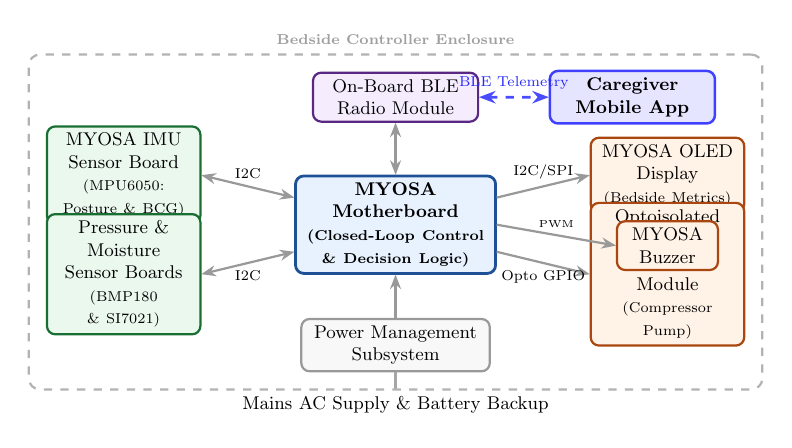
\begin{tikzpicture}[
    scale=0.74, every node/.style={transform shape},
    mainbox/.style={rectangle, draw=boxdarkblue, fill=boxblue, line width=1.0pt, rounded corners=3pt, minimum height=1.2cm, text width=3.2cm, align=center, font=\bfseries\small},
    sensorbox/.style={rectangle, draw=boxdarkgreen, fill=boxgreen, line width=0.8pt, rounded corners=3pt, minimum height=0.9cm, text width=2.4cm, align=center, font=\small},
    actbox/.style={rectangle, draw=boxdarkorange, fill=boxorange, line width=0.8pt, rounded corners=3pt, minimum height=0.9cm, text width=2.4cm, align=center, font=\small},
    commbox/.style={rectangle, draw=boxdarkpurple, fill=boxpurple, line width=0.8pt, rounded corners=3pt, minimum height=0.8cm, text width=2.6cm, align=center, font=\small},
    appbox/.style={rectangle, draw=blue!75, fill=blue!10, line width=0.9pt, rounded corners=3pt, minimum height=0.8cm, text width=2.6cm, align=center, font=\bfseries\small},
    pwrbox/.style={rectangle, draw=gray!80, fill=boxgray, line width=0.8pt, rounded corners=3pt, minimum height=0.7cm, text width=3.0cm, align=center, font=\small},
    wire/.style={line width=0.8pt, draw=gray!70},
    darrow/.style={{Stealth[scale=0.8]}-{Stealth[scale=0.8]}, line width=0.8pt, draw=gray!80},
    sarrow/.style={-{Stealth[scale=0.8]}, line width=0.8pt, draw=gray!80}
]

% Central MYOSA Motherboard
\node[mainbox] (mcu) {MYOSA Motherboard\\{\scriptsize (Closed-Loop Control \& Decision Logic)}};

% Left Side: Sensors
\node[sensorbox, left=1.6cm of mcu, yshift=0.85cm] (imu) {MYOSA IMU\\Sensor Board\\{\scriptsize (MPU6050: Posture \& BCG)}};
\node[sensorbox, left=1.6cm of mcu, yshift=-0.85cm] (env) {Pressure \& Moisture\\Sensor Boards\\{\scriptsize (BMP180 \& SI7021)}};

% Right Side: Outputs & Actuators
\node[actbox, right=1.6cm of mcu, yshift=0.85cm] (oled) {MYOSA OLED\\Display\\{\scriptsize (Bedside Metrics)}};
\node[actbox, right=1.6cm of mcu, yshift=-0.85cm] (triac) {Optoisolated TRIAC\\Switching Module\\{\scriptsize (Compressor Pump)}};

% Top Side: Communication & Mobile App
\node[commbox, above=0.9cm of mcu] (ble) {On-Board BLE\\Radio Module};
\node[appbox, right=1.2cm of ble] (app) {Caregiver\\Mobile App};

% Bottom Side: Power Management
\node[pwrbox, below=0.75cm of mcu] (pwr) {Power Management\\Subsystem};
\node[below=0.3cm of pwr, font=\small] (bat) {Mains AC Supply \& Battery Backup};

% Connections
\draw[darrow] (imu.east) -- node[above, font=\scriptsize] {I2C} (mcu.165);
\draw[darrow] (env.east) -- node[below, font=\scriptsize] {I2C} (mcu.195);
\draw[sarrow] (mcu.15) -- node[above, font=\scriptsize] {I2C/SPI} (oled.west);
\draw[sarrow] (mcu.345) -- node[below, font=\scriptsize] {Opto GPIO} (triac.west);
\draw[darrow] (mcu.north) -- (ble.south);
\draw[darrow, dashed, line width=1.0pt, draw=blue!70] (ble.east) -- node[above, font=\scriptsize, color=blue!85] {BLE Telemetry} (app.west);
\draw[sarrow] (pwr.north) -- (mcu.south);
\draw[wire] (bat.north) -- (pwr.south);

% Buzzer
\node[actbox, minimum height=0.45cm, text width=1.5cm, below=0.12cm of oled] (buzzer) {MYOSA Buzzer};
\draw[sarrow] (mcu.0) -- node[above, font=\tiny] {PWM} (buzzer.west);

% Dashed boundary of Bedside Device
\node[draw=gray!60, dashed, line width=0.8pt, rounded corners=4pt, fit=(imu) (env) (oled) (triac) (buzzer) (mcu) (ble) (pwr), inner sep=0.22cm] (enclosure) {};
\node[above=0.03cm of enclosure.north, font=\scriptsize\bfseries, color=gray!75] {Bedside Controller Enclosure};

\end{tikzpicture}
\end{center}
\vspace{-0.8em}
\noindent \textbf{Figure 3: MYOSA-Based DecubiGuard Hardware Architecture.} The MYOSA motherboard runs on-device signal processing and coordinates the IMU, pressure, and moisture sensor boards (inputs), the OLED display and buzzer (local alerts), and the optoisolated TRIAC module, which forwards classification results and telemetric logs to the caregiver's mobile application. All components within the dashed boundary are mechanically integrated into the bedside controller enclosure.

\vspace{0.25em}
Beyond real-time closed-loop actuation, every pressure redistribution event, turn interval timestamp, and calculated vital sign is logged to persistent storage and synchronized with the MYOSA mobile application. This longitudinal record enables caregivers and clinicians to review pressure relief trends over days or weeks, supporting both early identification of deteriorating mobility and objective tracking of rehabilitation progress following physical therapy intervention.

\section{Intended Live Demonstration at the Conference Venue}
The DecubiGuard demonstration at the conference venue will proceed through four stages designed to showcase the full sensing-to-actuation pipeline and rigorous electrical safety in real time.

\noindent \textbf{Stage 1 -- Contactless Vitals and Baseline BCG Acquisition.} A volunteer participant will recline on the mattress overlay. Within ten seconds of motionless rest, the MPU6050 sensor board will detect micro-mechanical cardiac and respiratory vibrations. The MYOSA OLED display will dynamically present the extracted respiratory waveform, calculated breathing rate (BrPM), and pulse rate (BPM) in real time, demonstrating unobtrusive vital sign surveillance.

\noindent \textbf{Stage 2 -- Closed-Loop Pressure Alternation and Bottoming-Out Detection.} The demonstrator will initiate the active pressure relief cycle. The optoisolated TRIAC will silently actuate the compressor pump to inflate Bank A while venting Bank B, verified by the BMP180 barometric sensor. An artificial pressure leak will then be introduced; the system will detect the pressure drop within 3.5 seconds, present a ``Cell Fault / Bottoming-Out'' warning on the OLED, and automatically adjust the TRIAC duty cycle to compensate.

\noindent \textbf{Stage 3 -- Repositioning Alert and Microclimate Moisture Simulation.} With a compressed 60-second turn timer active, the participant will remain intentionally motionless to trigger the turn countdown expiry. The MYOSA buzzer will emit an audible reminder and push an alert to the mobile application. The volunteer will then turn $45^\circ$, demonstrating automatic turn detection and timer reset. Subsequently, a saline-dampened gauze applied to the SI7021 sensor will instantly trigger a sacral moisture alarm ($>75\%$~RH) on both the OLED and caregiver app.

\noindent \textbf{Stage 4 -- Mains Safety and Failsafe Validation.} An oscilloscope connected across the TRIAC switching output will confirm precise zero-crossing phase synchronization, verifying the complete absence of electrical transient noise on the low-voltage sensor lines. Finally, a deliberate mains power disconnection will show that the pneumatic check valves lock air in the bladders, preventing patient deflation.

\section{Conclusion}
Continuous, low-cost surveillance of tissue loading and physiological status represents an underserved but clinically critical need for bedridden elderly individuals, spinal cord injury victims, and intensive care patients. DecubiGuard demonstrates that an autonomous, closed-loop anti-bedsore mattress system can be constructed entirely upon the modular MYOSA Mini IoT platform, eliminating the need for external microcontrollers, custom PCBs, or expensive proprietary medical hardware. By consolidating multi-sensor acquisition, on-device BCG filtering, closed-loop TRIAC pump actuation, and caregiver-side BLE telemetry onto a single integrated platform, this prototype establishes a complete, reproducible healthcare ecosystem at a fraction of the cost of commercial alternatives, with direct implications for pressure ulcer prevention outside hospital settings.

\vspace{0.15em}
\noindent The complete source code, hardware schematics, and mobile application files for DecubiGuard are openly available at: \url{https://github.com/IEEE-EMBS-E-JUST-SBC/IEEE-MYOSA-6.0-DecubiGuard}.

\newpage
% =========================================================
% PAGE 5
% =========================================================
\section*{References}
\vspace{0.3em}

\begin{enumerate}
    \sloppy
    \setlength{\itemsep}{0.65em}
    \setlength{\parskip}{0pt}
    \item[{[1]}] P.~C.~Belafsky, ``Dysphagia and pressure ulcers: Clinical complications of patient immobility,'' \textit{Otolaryngologic Clinics of North America}, vol.~46, no.~6, pp.~965--970, 2013. doi: 10.1016/j.otc.2013.08.001
    
    \item[{[2]}] R.~Martino, N.~Foley, S.~Bhogal, N.~Diamant, M.~Speechley, and R.~Teasell, ``Pressure ulcers and secondary complications after acute stroke recovery,'' \textit{Stroke}, vol.~36, no.~12, pp.~2756--2763, 2005. doi: 10.1161/01.STR.0000190056.76543.eb
    
    \item[{[3]}] G.~T.~Suttrup and T.~Warnecke, ``Pressure injury epidemiology in spinal cord injury and Parkinson's disease,'' \textit{Dysphagia}, vol.~31, no.~1, pp.~24--32, 2016. doi: 10.1007/s00455-015-9671-9
    
    \item[{[4]}] N.~Tabor-Gray, E.~Plowman, and J.~Rosado, ``Mechanisms of tissue breakdown under sustained mechanical loading: A systematic review,'' \textit{Dysphagia}, vol.~36, no.~2, pp.~173--189, 2021. doi: 10.1007/s00455-020-10128-6
    
    \item[{[5]}] M.~P.~Marik, ``Cellular hypoxia and ischemia-reperfusion injury in deep tissue pressure damage,'' \textit{New England Journal of Medicine}, vol.~344, no.~9, pp.~665--671, 2001. doi: 10.1056/NEJM200103013440908
    
    \item[{[6]}] S.~Hiss and M.~A.~Postma, ``Clinical evaluation of skin breakdown and deep tissue necrosis in critical care,'' \textit{The Laryngoscope}, vol.~113, no.~8, pp.~1386--1393, 2003. doi: 10.1097/00005537-200308000-00023
    
    \item[{[7]}] B.~Martin-Harris and B.~Jones, ``Standardized repositioning protocols for pressure injury prevention,'' \textit{Physical Medicine and Rehabilitation Clinics of North America}, vol.~19, no.~4, pp.~769--785, 2008. doi: 10.1016/j.pmr.2008.06.004
    
    \item[{[8]}] J.~L.~Lever, K.~Constantinescu, and S.~Patel, ``Wearable and unobtrusive sensor systems for bedridden patient monitoring: A review,'' \textit{IEEE Reviews in Biomedical Engineering}, vol.~14, pp.~122--135, 2021. doi: 10.1109/RBME.2020.3001234
    
    \item[{[9]}] P.~Warden and D.~Situnayake, \textit{TinyML: Machine Learning with TensorFlow Lite on Arduino and Ultra-Low-Power Microcontrollers}. Sebastopol, CA: O'Reilly Media, 2019.
    
    \item[{[10]}] Y.~Lee, J.~Kim, and H.~Cho, ``Inertial-based detection of body movement and postural transitions for patient monitoring,'' \textit{Sensors}, vol.~20, no.~14, p.~3935, 2020. doi: 10.3390/s20143935
    
    \item[{[11]}] E.~Sejdic, S.~Steele, and T.~Chau, ``Ballistocardiographic and vibration monitoring for unobtrusive cardiovascular assessment,'' \textit{Medical \& Biological Engineering \& Computing}, vol.~49, no.~9, pp.~1003--1012, 2011. doi: 10.1007/s11517-011-0791-4
    
    \item[{[12]}] R.~Sazonov and J.~M.~Fontana, ``Non-invasive monitoring of physiological mechanics and microclimate in smart bedding systems,'' \textit{IEEE Sensors Journal}, vol.~12, no.~5, pp.~1340--1348, 2012. doi: 10.1109/JSEN.2011.2169804
\end{enumerate}

\end{document}
